\documentclass[twocolumn,fontsize=11pt]{scrartcl}

% Basic packages
\usepackage[utf8]{inputenc}
\usepackage[T1]{fontenc}
\usepackage{lmodern}
\usepackage[a4paper,margin=1.5cm]{geometry}
\usepackage{multicol}
\usepackage{graphicx}
\usepackage{caption}
\usepackage{subcaption}
\usepackage{amsmath,amssymb}
\usepackage{siunitx}
\usepackage{booktabs}
\usepackage{physics}
\usepackage{float}
\usepackage{hyperref}
\usepackage{physics_macros} % Your custom macros
\usepackage{biblatex} % For bibliography
\addbibresource{bibliography.bib}

% Header and footer
\usepackage{fancyhdr}
\pagestyle{fancy}
\fancyhf{}
\lhead{Star and Stellar Evolution}
\rhead{\thepage}

%Folder
\graphicspath{{plots/}}

% Title
\title{\vspace{-1cm}Stellar Structure Evolution with MESA}
\author{Bruno da Rocha Schultz}
\date{\today}

\begin{document}
\maketitle

\section*{Exercise 1}

\paragraph{Q.1.1:} Why is there only one history file but multiple profile files?

\paragraph{A:} The history file contains the global properties of the star at each time step, while the profile files contain the detailed structure of the star at specific points in time. The history file is updated at each time step, but the profile files are only written at certain intervals. So there is one history file for the entire simulation, but multiple profile files corresponding to different time steps.

\paragraph{Q.1.2:} Show with a plot whether or not the size of the time steps in the history file changes
during the simulation, and discuss why.

\paragraph{A:} The time steps in the history file do change during the simulation. This is because MESA uses an adaptive time-stepping algorithm to ensure that the simulation progresses at a rate that captures the important changes in the star's structure and evolution. The time steps are smaller during rapid changes (like during a shell flash) and larger during more stable phases. Cf. Figure \ref{fig:time_steps} for a plot of the time steps recorded in the history file. 

\begin{figure}[htbp]
    \centering
    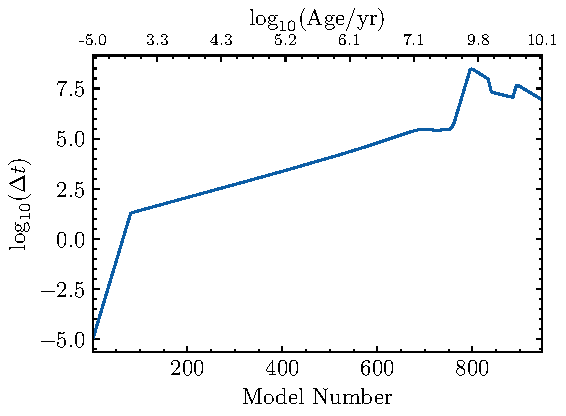
\includegraphics{log_dt_vs_model_number.pdf}
    \caption{Time steps recorded in the history file. The x-axis shows the model number (bottom) and the logarithm of the stellar age (top). The y-axis shows the logarithm of the time step size.}
    \label{fig:time_steps}
\end{figure}

\paragraph{Q.1.3:} Similarly, show with a plot whether or not the grid spacing in a profile file of your
choice is constant, and discuss why. From this plot, also infer which zone is the most  
central zone (zone number 1 or the zone with the highest number).

\paragraph{A:} The grid spacing in a profile file is not constant. MESA uses a non-uniform grid so it can better capture important changes inside the star, making the grid finer where the structure changes quickly and coarser where things are more uniform. In Figure \ref{fig:grid_spacing}, the top graph shows that zone number 1 is at the surface, while the highest zone number is at the center. The bottom graph shows that the spacing between zones (measured as \(\log_{10}(\Delta R / R)\)) is not the same everywhere, confirming that the grid is not evenly spaced. Here, \(\Delta R\) is the difference in radius between adjacent zones, i.e. \(\Delta R = R_{i+1} - R_i\).


\begin{figure}[htbp]
    \centering
    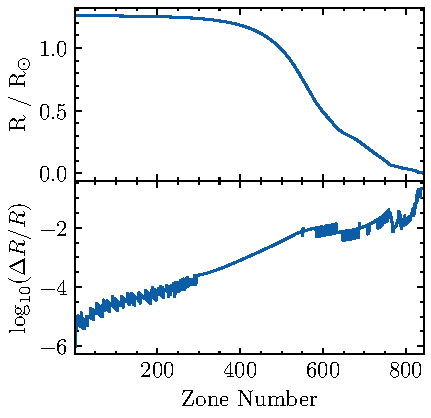
\includegraphics{R_vs_zone.pdf}
    \caption{Grid spacing in a profile file. The x-axis shows the zone number. Top: The radius of each zone.}
    \label{fig:grid_spacing}
\end{figure}


\paragraph{Q.1.4:} Which burning stages did the simulation go through, and where did that burning take
place? Graphically Illustrate your answer

\printbibliography

\end{document}
